
\item Four charges $Q_1$, $Q_2$, $Q_3$ and $Q_4$ of same magnitude are fixed along the x axis at $x = -2a$, $-a$, $+a$ and $+2a$, respectively. A positive charge $q$ is placed on the positive y axis at a distance $b > 0$. Four options of the signs of these charges are given in List I. The direction of the forces on the charge $q$ is given in List II. Match List I with List II and select the correct answer using the code given below the lists.

\begin{center}
    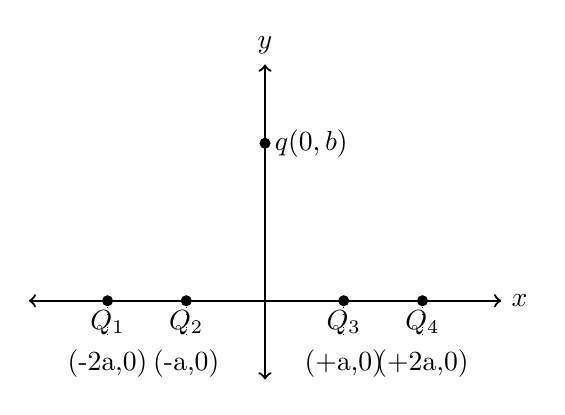
\begin{tikzpicture}
        \draw[<->,thick] (-3,0)--(3,0) node[right]{$x$};
        \draw[<->,thick] (0,-1)--(0,3) node[above]{$y$};
        
        \fill (-2,0) circle (2pt) node[below] {$Q_1$};
        \fill (-1,0) circle (2pt) node[below] {$Q_2$};
        \fill (1,0) circle (2pt) node[below] {$Q_3$};
        \fill (2,0) circle (2pt) node[below] {$Q_4$};
        \fill (0,2) circle (2pt) node[right] {$q (0,b)$};

        \draw[dotted] (-2,0) -- (-2,-0.5) node[below] {(-2a,0)};
        \draw[dotted] (-1,0) -- (-1,-0.5) node[below] {(-a,0)};
        \draw[dotted] (1,0) -- (1,-0.5) node[below] {(+a,0)};
        \draw[dotted] (2,0) -- (2,-0.5) node[below] {(+2a,0)};
    \end{tikzpicture}
\end{center}

\begin{center}
    \renewcommand{\arraystretch}{1.5}
    \begin{table}[h]
        \centering
        \begin{tabular}{p{0.25cm}p{8cm}|p{0.25cm}p{5cm}}
        \hline
        & List I & & List II \\
        \hline
        P & $Q_1, Q_2, Q_3, Q_4$ all positive & 1 & $+x$ \\
        Q & $Q_1, Q_2$ positive; $Q_3, Q_4$ negative & 2 & $-x$ \\
        R & $Q_1, Q_4$ positive; $Q_2, Q_3$ negative & 3 & $+y$ \\
        S & $Q_1, Q_3$ positive; $Q_2, Q_4$ negative & 4 & $-y$ \\
        \hline
        \end{tabular}
    \end{table}
\end{center}

\begin{tasks}(2)
    \task P-3, Q-1, R-4, S-2
    \task P-4, Q-2, R-3, S-1
    \task P-3, Q-1, R-2, S-4
    \task P-4, Q-2, R-1, S-3
\end{tasks}
